The vector equation of a line can be expressed as 
\begin{align}
    \vec{x} = \vec{q} +\mu\vec{m} \label{eq:solutions/4/2/8/vec_eqn_of_line}
\end{align}
The general equation of a second degree can be expressed as :
\begin{align}
\vec{x}^T\vec{V}\vec{x}+2\vec{u}^T\vec{x}+f=0\label{eq:solutions/4/2/8/gen__quad_eqn}
\end{align}

Comparing \eqref{eq:solutions/4/2/8/given_circle_eq} with \eqref{eq:solutions/4/2/8/gen__quad_eqn}
\begin{align}
\vec{u}=\myvec{-2 \\ \frac{-3}{2}}, f=5
\end{align}
If $\vec{n}$ is the normal vector of a line, equation of that line can be written as 
\begin{align}
\vec{n}^T\vec{x} = c \label{eq:solutions/4/2/8/eq1}
\end{align}
Comparing \eqref{eq:solutions/4/2/8/given_line_eq} with \eqref{eq:solutions/4/2/8/eq1}
\begin{align}
\vec{n} = \myvec{1 \\ 1}\label{eq:solutions/4/2/8/eq2}
\end{align}
Since it is mentioned that the tangent is parallel to given line it will have same normal vector. \\
 The point of contact $\vec{q}$, of a line with a normal vector $\vec{n}$ to the conic in \eqref{eq:solutions/4/2/8/gen__quad_eqn} is given by:
\begin{align}
\vec{q} = \vec{V}^{-1}\brak{\kappa \vec{n}-\vec{u}} \label{eq:solutions/4/2/8/eq3} \\
\kappa = \pm \sqrt{\frac{\vec{u}^T\vec{V}^{-1}\vec{u}-f}{\vec{n}^T\vec{V}^{-1}\vec{n}}} \label{eq:solutions/4/2/8/eq4}
\end{align}
The point of contact $\vec{q}$, of a line with a normal vector $\vec{n}$ to the conic in \eqref{eq:solutions/4/2/8/gen__quad_eqn} is given by:
\begin{align}
\vec{q} = \vec{V}^{-1}\brak{\kappa \vec{n}-\vec{u}} 
%\label{eq:solutions/4/2/8/eq3}
 \\
\kappa = \pm \sqrt{\frac{\vec{u}^T\vec{V}^{-1}\vec{u}-f}{\vec{n}^T\vec{V}^{-1}\vec{n}}} 
%\label{eq:solutions/4/2/8/eq4}
\end{align}
We know that, for a circle, 
\begin{align}
\vec{V} = \vec{I}  
\end{align}
and from the properties of an Identity matrix, 
\begin{align}
\vec{I}^{-1} &= \vec{I} \\
\vec{I}\vec{X} &= \vec{X}   
\end{align}
Solving for the point of contact using the above equations we get,
\begin{align}
\kappa &= \pm \sqrt{\frac{\myvec{ -2 & -1.5 }\myvec{-2 \\ -1.5} - 5}{\myvec{1 & 1 }\myvec{1 \\ 1 }}} \\
&= \pm \sqrt{\frac{6.25 - 5}{2}} \\
& =  \pm \sqrt{\frac{5}{8}}\\
\end{align}
So there are two tangents to a circle which are parallel to given line which touch circle at two different points  $\vec{q_1}$ and $\vec{q_2}$
\begin{align}
\vec{q_1} &= \myvec{\sqrt{\frac{5}{8}} \\ \sqrt{\frac{5}{8}}} + \myvec{2 \\ \frac{3}{2}} \\
&= \myvec{\frac{279}{100} \\ \frac{229}{100}}
\end{align}
\begin{align}
\vec{q_2} &= \myvec{-\sqrt{\frac{5}{8}} \\ \sqrt{\frac{5}{8}}} + \myvec{2 \\ \frac{3}{2}} \\
&= \myvec{\frac{121}{100} \\ \frac{71}{100}}
\end{align}
Since points $\vec{q_1}$ and $\vec{q_2}$ lie on tangent they satisfy the line equation of tangents, there are two different tangents with same normal vector
\begin{align}
\vec{n}^T\vec{q_1} = c_1 
%\label{eq:solutions/4/2/8/eq1}
\end{align}
\begin{align}
\vec{n}^T\vec{q_2} = c_2 
%\label{eq:solutions/4/2/8/eq1}
\end{align}
$c_1$ and $c_2$ are some constants
\begin{align}
c_1=\myvec{1 & 1}\myvec{\frac{279}{100} \\ \frac{229}{100}}\newline
&= \frac{127}{25}
\end{align}
\newline
\begin{align}
c_2=\myvec{\frac{121}{100} \\ \frac{71}{100}}\newline
&= \frac{48}{25}
\end{align}
So line equations of tangents to the given circle which are parallel to line are
\begin{align}
\myvec{1 &1}\vec{x}=\frac{127}{25}
\end{align}and
\newline
\begin{align}
\myvec{1 &1}\vec{x}=\frac{48}{25}
\end{align}
%
\begin{figure}[]
\centering
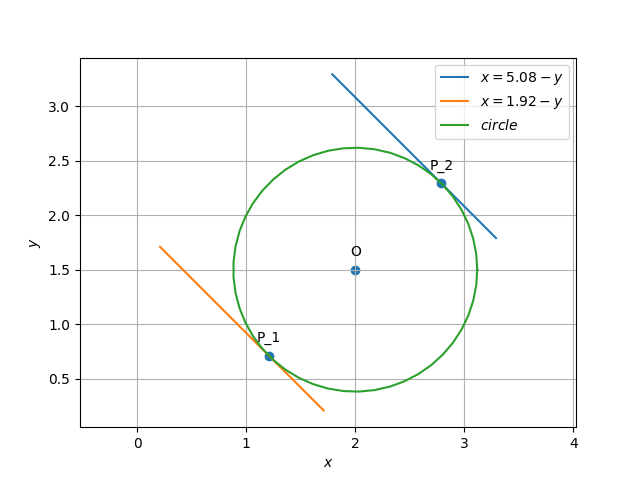
\includegraphics[width=\columnwidth]{./solutions/4/2/8/Figure_1.png}
\caption{Circle with center (2 1.5) and having the lines (1 1)x =5.08 and (1 1)x =1.92 as tangents with (2.79 2.29) and (1.21 0.71) as point of contact.}
\label{eq:solutions/4/2/8/Fig:Circle}
\end{figure}

